\subsubsection{x86}

\myparagraph{\NonOptimizing MSVC}

Это дает в итоге (MSVC 2010):

\lstinputlisting[caption=MSVC 2010]{patterns/08_switch/1_few/few_msvc.asm}

Наша функция со оператором switch(), с небольшим количеством вариантов, 
это практически аналог подобной конструкции:

\lstinputlisting[label=switch_few_ifelse]{patterns/08_switch/1_few/few_analogue.c}

\myindex{\CLanguageElements!switch}
\myindex{\CLanguageElements!if}
Когда вариантов немного и мы видим подобный код, невозможно сказать с уверенностью, был ли
в оригинальном исходном коде switch(), либо просто набор операторов if().

\myindex{\SyntacticSugar}
То есть, switch() это синтаксический сахар для большого количества вложенных проверок 
при помощи if().

В самом выходном коде ничего особо нового, 
за исключением того, что компилятор зачем-то 
перекладывает входящую переменную ($a$) во временную в локальном стеке \TT{v64}\footnote{Локальные переменные в стеке с префиксом \TT{tv}~--- 
так MSVC называет внутренние переменные для своих нужд}.

Если скомпилировать это при помощи GCC 4.4.1, то будет почти то же самое, даже с максимальной оптимизацией (ключ \Othree).

\myparagraph{\Optimizing MSVC}

% TODO separate various kinds of \TT
% idea: enclose command lines in a specific environment, like \cmdline{} 
% assembly instructions in \asm{} (now both \TT and \q{} are used),
% variables in,  like \var{}
% messages (string constants) in something else, like \strconst
% to separate them all. Now they all use \TT, which is not best
% \INS{} for all instructions including operands? --DY

Попробуем включить оптимизацию кодегенератора MSVC (\Ox): \TT{cl 1.c /Fa1.asm /Ox}

\label{JMP_instead_of_RET}
\lstinputlisting[caption=MSVC]{patterns/08_switch/1_few/few_msvc_Ox.asm}

Вот здесь уже всё немного по-другому, причем не без грязных трюков.

\myindex{x86!\Instructions!JZ}
\myindex{x86!\Instructions!JE}
\myindex{x86!\Instructions!SUB}
Первое: \TT{а} помещается в \EAX и от него отнимается 0. Звучит абсурдно, но нужно это для того, чтобы проверить, 
0 ли в \EAX был до этого? Если да, то выставится флаг \ZF (что означает, что результат вычитания 0 от числа 
стал 0) и первый условный переход \JE (\IT{Jump if Equal} или его синоним \JZ~--- \IT{Jump if Zero}) 
сработает на метку \TT{\$LN4@f}, где выводится сообщение \TT{'zero'}.
Если первый переход не сработал, от значения отнимается по единице, 
и если на какой-то стадии в результате образуется 0, то сработает соответствующий переход.

И в конце концов, если ни один из условных переходов не сработал, управление передается \printf
со строковым аргументом \TT{'something unknown'}.

\label{jump_to_last_printf}
\myindex{\Stack}
Второе: мы видим две, мягко говоря, необычные вещи: указатель на сообщение помещается в переменную $a$, 
и затем \printf вызывается не через \CALL, а через \JMP. Объяснение этому простое. 
Вызывающая функция заталкивает в стек некоторое значение и через \CALL вызывает нашу функцию. 
\CALL в свою очередь заталкивает в стек адрес возврата (\ac{RA}) и делает безусловный переход на адрес нашей функции. 
Наша функция в самом начале (да и в любом её месте, потому что в теле функции нет ни одной инструкции, 
которая меняет что-то в стеке или в \ESP) имеет следующую разметку стека:

\begin{itemize}
\item\ESP --- хранится \ac{RA}
\item\TT{ESP+4} --- хранится значение $a$ 
\end{itemize}

С другой стороны, чтобы вызвать \printf, нам нужна почти такая же разметка стека, 
только в первом аргументе нужен указатель на строку. Что, собственно, этот код и делает.

Он заменяет свой первый аргумент на адрес строки, и затем передает управление \printf, как если бы вызвали не 
нашу функцию \ttf, а сразу \printf. 
\printf выводит некую строку на \gls{stdout}, затем исполняет инструкцию \RET, 
которая из стека достает \ac{RA} и управление передается в ту функцию, 
которая вызывала \ttf, минуя при этом конец функции \ttf.

\myindex{\CStandardLibrary!longjmp()}
\newcommand{\URLSJ}{\href{http://go.yurichev.com/17121}{wikipedia}}
Всё это возможно, потому что \printf вызывается в \ttf в самом конце. 
Всё это чем-то даже похоже на \TT{longjmp()}\footnote{\URLSJ}.
И всё это, разумеется, сделано для экономии времени исполнения.

Похожая ситуация с компилятором для ARM описана в секции \q{\PrintfSeveralArgumentsSectionName}~(\myref{ARM_B_to_printf}).

\clearpage
\myparagraphold{\olly}

Так как этот пример немного запутанный, попробуем оттрассировать его в \olly.

\olly может распознавать подобные switch()-конструкции, так что он добавляет полезные комментарии.
\EAX в начале равен 2, это входное значение функции: 

\begin{figure}[H]
\centering
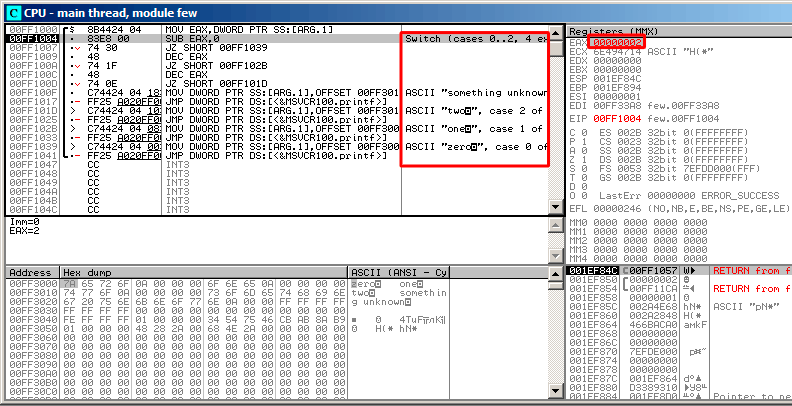
\includegraphics[scale=\FigScale]{patterns/08_switch/1_few/olly1.png}
\caption{\olly: \EAX содержит первый (и единственный) аргумент функции}
\label{fig:switch_few_olly1}
\end{figure}

\clearpage
0 отнимается от 2 в \EAX. 
Конечно же, \EAX всё ещё содержит 2.
Но флаг \ZF теперь 0, что означает, что последнее вычисленное значение не было нулевым:

\begin{figure}[H]
\centering
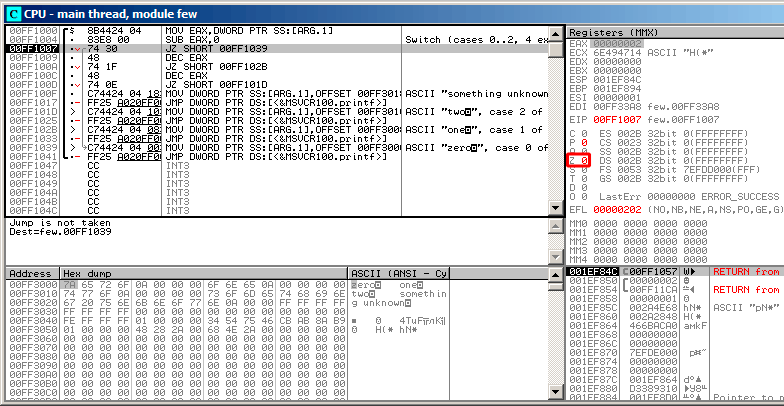
\includegraphics[scale=\FigScale]{patterns/08_switch/1_few/olly2.png}
\caption{\olly: \SUB исполнилась}
\label{fig:switch_few_olly2}
\end{figure}

\clearpage
\DEC исполнилась и \EAX теперь содержит 1. 
Но 1 не ноль, так что флаг \ZF всё ещё 0:

\begin{figure}[H]
\centering
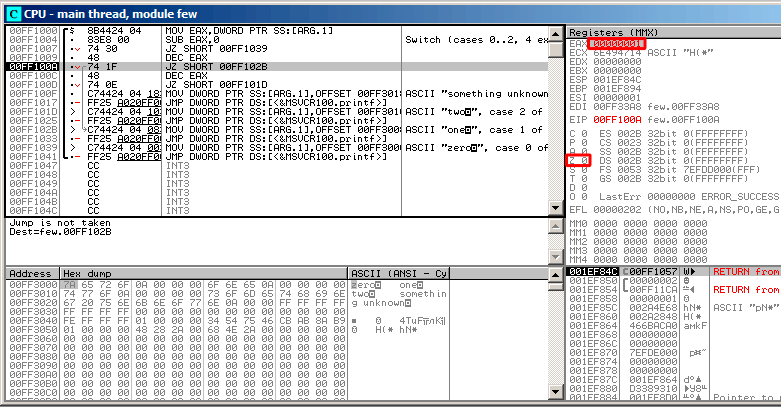
\includegraphics[scale=\FigScale]{patterns/08_switch/1_few/olly3.png}
\caption{\olly: первая \DEC исполнилась}
\label{fig:switch_few_olly3}
\end{figure}

\clearpage
Следующая \DEC исполнилась. 
\EAX наконец 0 и флаг \ZF выставлен, потому что результат~--- ноль:

\begin{figure}[H]
\centering
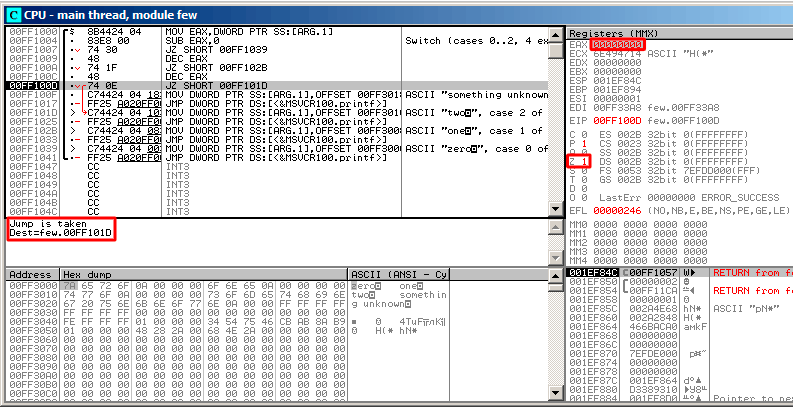
\includegraphics[scale=\FigScale]{patterns/08_switch/1_few/olly4.png}
\caption{\olly: вторая \DEC исполнилась}
\label{fig:switch_few_olly4}
\end{figure}

\olly показывает, что условный переход сейчас сработает.

\clearpage
Указатель на строку \q{two} 
сейчас будет записан в стек:

\begin{figure}[H]
\centering
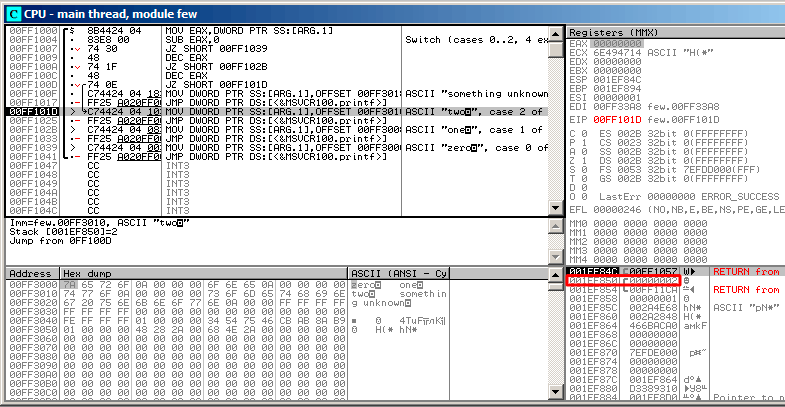
\includegraphics[scale=\FigScale]{patterns/08_switch/1_few/olly5.png}
\caption{\olly: указатель на строку сейчас запишется на место первого аргумента}
\label{fig:switch_few_olly5}
\end{figure}

% TODO: homogenize numbers
% now they are inconsistent: sometimes plain text, sometimes in math mode
% some kind of \expr{} both for numbers and expressions? --DY
Обратите внимание: текущий аргумент функции это 2 и 2 прямо сейчас в стеке по адресу \TT{0x001EF850}.

\clearpage
\MOV записывает указатель на строку по адресу \TT{0x001EF850} (см. окно стека).
Переход сработал.
Это самая первая инструкция функции \printf в MSVCR100.DLL (этот пример был скомпилирован с опцией /MD): 

\begin{figure}[H]
\centering
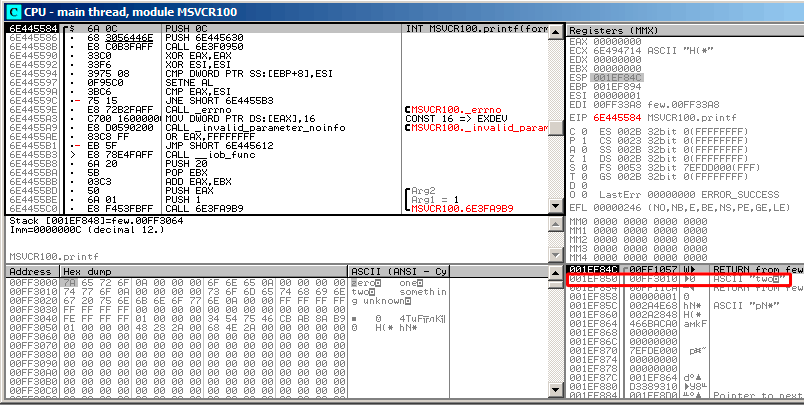
\includegraphics[scale=\FigScale]{patterns/08_switch/1_few/olly6.png}
\caption{\olly: первая инструкция в \printf в MSVCR100.DLL}
\label{fig:switch_few_olly6}
\end{figure}

Теперь \printf считает строку на \TT{0x00FF3010} как свой единственный аргумент и выводит строку.

\clearpage
Это самая последняя инструкция функции \printf:

\begin{figure}[H]
\centering
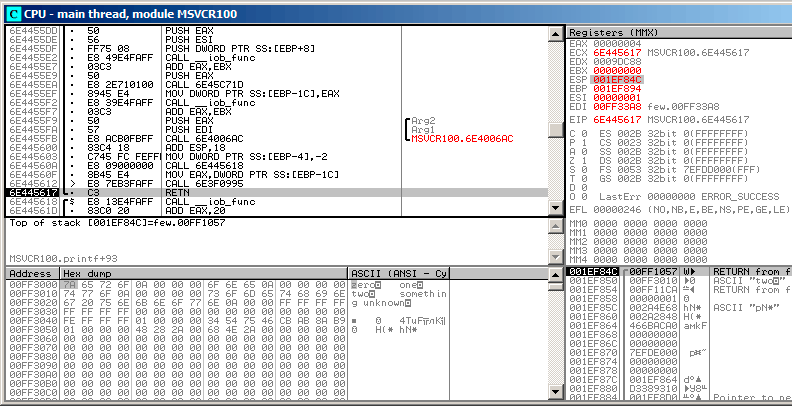
\includegraphics[scale=\FigScale]{patterns/08_switch/1_few/olly7.png}
\caption{\olly: последняя инструкция в \printf в MSVCR100.DLL}
\label{fig:switch_few_olly7}
\end{figure}

Строка \q{two} была только что выведена в консоли.

\clearpage
Нажмем F7 или F8 (\stepover) и вернемся\dots нет, не в функцию \ttf но в \main:

\begin{figure}[H]
\centering
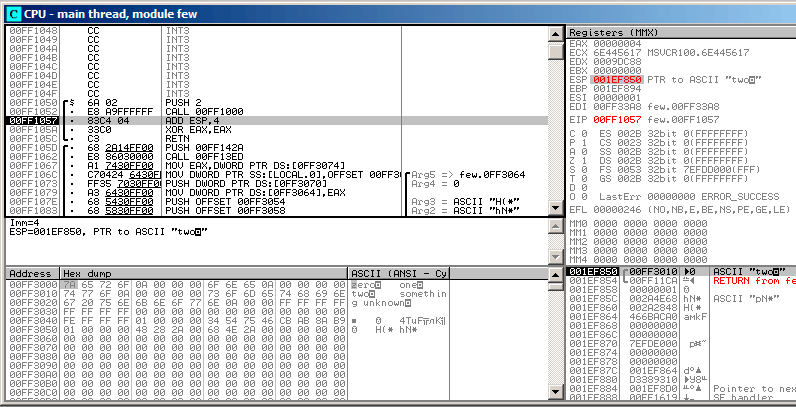
\includegraphics[scale=\FigScale]{patterns/08_switch/1_few/olly8.png}
\caption{\olly: возврат в \main}
\label{fig:switch_few_olly8}
\end{figure}

Да, это прямой переход из внутренностей \printf в \main.
Потому как \ac{RA} в стеке указывает не на какое-то место в функции \ttf а в \main.
И \CALL \TT{0x00FF1000} это инструкция вызывающая функцию \ttf.



